\documentclass{article}
\usepackage{tikz,pgfplots}
% and optionally (as of Pgfplots 1.3):
\pgfplotsset{compat=newest}
\pgfplotsset{plot coordinates/math parser=false}
%\newlength\figureheight
%\newlength\figurewidth

\begin{document}
% Setting the figure dimensions is optional (see above).
%\setlength\figureheight{2cm}
%\setlength\figurewidth{3cm}

This is my first figure, \\
% This file was created by matlab2tikz v0.3.2.
% Copyright (c) 2008--2013, Nico Schlömer <nico.schloemer@gmail.com>
% All rights reserved.
% 
% The latest updates can be retrieved from
%   http://www.mathworks.com/matlabcentral/fileexchange/22022-matlab2tikz
% where you can also make suggestions and rate matlab2tikz.
% 
% 
% 
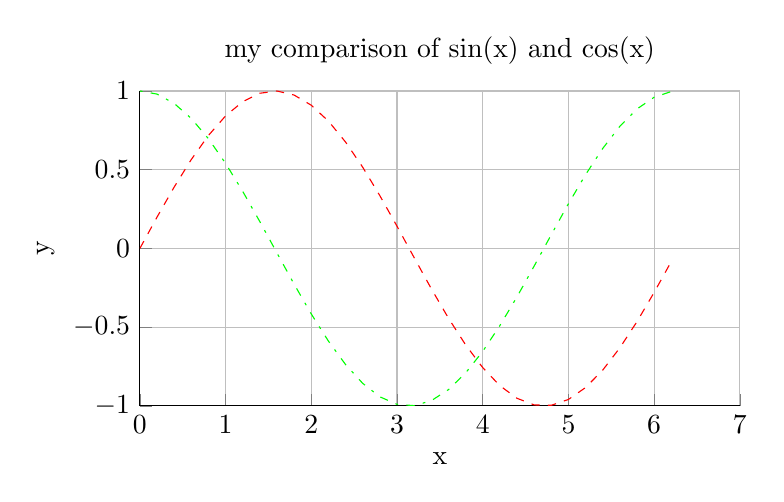
\begin{tikzpicture}

\begin{axis}[%
width=3in,
height=4cm,
scale only axis,
xmin=0, xmax=7,
xlabel={x},
xmajorgrids,
ymin=-1, ymax=1,
ylabel={y},
ymajorgrids,
title={my comparison of sin(x) and cos(x)},
axis x line*=bottom,
axis y line*=left
]
\addplot [
color=red,
dashed,
forget plot
]
table{
0 0
0.2 0.198669330795061
0.4 0.389418342308651
0.6 0.564642473395035
0.8 0.717356090899523
1 0.841470984807897
1.2 0.932039085967226
1.4 0.98544972998846
1.6 0.999573603041505
1.8 0.973847630878195
2 0.909297426825682
2.2 0.80849640381959
2.4 0.675463180551151
2.6 0.515501371821464
2.8 0.334988150155905
3 0.141120008059867
3.2 -0.0583741434275801
3.4 -0.255541102026831
3.6 -0.442520443294852
3.8 -0.611857890942719
4 -0.756802495307928
4.2 -0.871575772413588
4.4 -0.951602073889516
4.6 -0.993691003633464
4.8 -0.996164608835841
5 -0.958924274663138
5.2 -0.883454655720153
5.4 -0.772764487555987
5.6 -0.631266637872322
5.8 -0.464602179413757
6 -0.279415498198926
6.2 -0.0830894028174964
};
\addplot [
color=green,
dash pattern=on 1pt off 3pt on 3pt off 3pt,
forget plot
]
table{
0 1
0.2 0.980066577841242
0.4 0.921060994002885
0.6 0.825335614909678
0.8 0.696706709347165
1 0.54030230586814
1.2 0.362357754476673
1.4 0.169967142900241
1.6 -0.0291995223012888
1.8 -0.227202094693087
2 -0.416146836547142
2.2 -0.588501117255346
2.4 -0.737393715541246
2.6 -0.856888753368947
2.8 -0.942222340668658
3 -0.989992496600445
3.2 -0.998294775794753
3.4 -0.966798192579461
3.6 -0.896758416334147
3.8 -0.790967711914417
4 -0.653643620863612
4.2 -0.490260821340699
4.4 -0.307332869978419
4.6 -0.112152526935055
4.8 0.0874989834394464
5 0.283662185463226
5.2 0.468516671300377
5.4 0.634692875942635
5.6 0.77556587851025
5.8 0.885519516941319
6 0.960170286650366
6.2 0.996542097023218
};
\end{axis}
\end{tikzpicture}% 

This is my second figure, \\
% This file was created by matlab2tikz v0.3.2.
% Copyright (c) 2008--2013, Nico Schlömer <nico.schloemer@gmail.com>
% All rights reserved.
% 
% The latest updates can be retrieved from
%   http://www.mathworks.com/matlabcentral/fileexchange/22022-matlab2tikz
% where you can also make suggestions and rate matlab2tikz.
% 
% 
% 
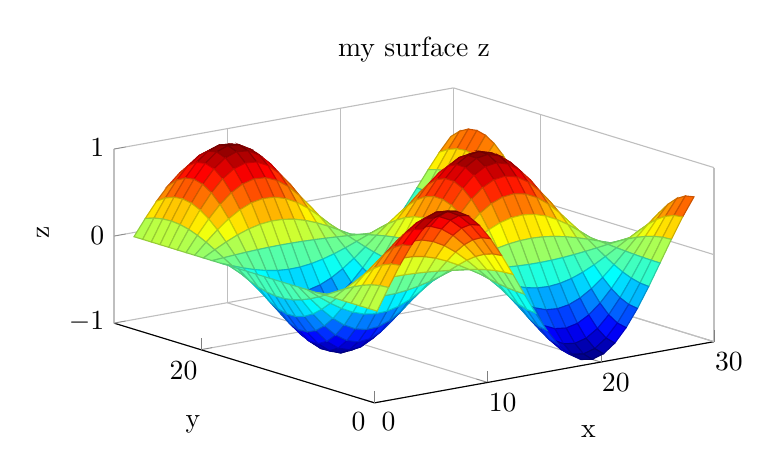
\begin{tikzpicture}

\begin{axis}[%
width=3in,
height=4cm,
view={-37.5}{30},
scale only axis,
xmin=0, xmax=30,
xlabel={x},
xmajorgrids,
ymin=0, ymax=30,
ylabel={y},
ymajorgrids,
zmin=-1, zmax=1,
zlabel={z},
zmajorgrids,
title={my surface z},
axis x line*=bottom,
axis y line*=left,
axis z line*=left
]

\addplot3[%
surf,
colormap/jet,
shader=faceted,
draw=black,
mesh/rows=29]
table[header=false] {
1 1 0
1 2 0
1 3 0
1 4 0
1 5 0
1 6 0
1 7 0
1 8 0
1 9 0
1 10 0
1 11 0
1 12 0
1 13 0
1 14 0
1 15 0
1 16 0
1 17 0
1 18 0
1 19 0
1 20 0
1 21 0
1 22 0
1 23 0
1 24 0
1 25 0
1 26 0
1 27 0
1 28 0
1 29 0
2 1 0.247403959254523
2 2 0.239712769302102
2 3 0.217117400384406
2 4 0.181022723101847
2 5 0.133672929666126
2 6 0.078012000898079
2 7 0.0175006637591753
2 8 -0.0440987798891864
2 9 -0.102956374993008
2 10 -0.155412641360863
2 11 -0.198206102417795
2 12 -0.228676068022045
2 13 -0.24492806329122
2 14 -0.245951617874744
2 15 -0.231683092106118
2 16 -0.203009633809154
2 17 -0.16171401974312
2 18 -0.110363811178584
2 19 -0.0521517153733972
2 20 0.00930292150097929
2 21 0.070179147774393
2 22 0.126691974546373
2 23 0.175327707963667
2 24 0.213062413685733
2 25 0.237549930475851
2 26 0.247267743143371
2 27 0.241611645164087
2 28 0.220933305315487
2 29 0.186518402615444
3 1 0.479425538604203
3 2 0.464521359638929
3 3 0.420735492403948
3 4 0.350790330050532
3 5 0.259034723999926
3 6 0.151173593425301
3 7 0.0339132210088926
3 8 -0.0854557112338325
3 9 -0.199511421250049
3 10 -0.301162477410803
3 11 -0.384088709382907
3 12 -0.443134165709015
3 13 -0.474627685896788
3 14 -0.476611155397338
3 15 -0.448961251683898
3 16 -0.393397111849238
3 17 -0.313373444987739
3 18 -0.213865735116517
3 19 -0.101060889677605
3 20 0.0180274324009957
3 21 0.135994896047353
3 22 0.24550685573806
3 23 0.339754388232106
3 24 0.412877638439518
3 25 0.460330156829104
3 26 0.479161575639938
3 27 0.468201048458857
3 28 0.428130047779531
3 29 0.361439994343462
4 1 0.681638760023334
4 2 0.66044826170605
4 3 0.598194289305055
4 4 0.498747493302027
4 5 0.368290993809707
4 6 0.214935944110739
4 7 0.0482172184322935
4 8 -0.12149942035197
4 9 -0.283661813651627
4 10 -0.428187489272094
4 11 -0.546090540702023
4 12 -0.630040327257651
4 13 -0.674817257815132
4 14 -0.677637319705942
4 15 -0.638325175140458
4 16 -0.559325062862482
4 17 -0.445548827222635
4 18 -0.304070523486759
4 19 -0.143686587342124
4 20 0.0256310848687682
4 21 0.193355140364663
4 22 0.349057309733086
4 23 0.483056786213911
4 24 0.587022131375477
4 25 0.654489283603605
4 26 0.68126346214459
4 27 0.665679978255382
4 28 0.608707737486832
4 29 0.513888997829366
5 1 0.841470984807897
5 2 0.81531168968946
5 3 0.738460262604129
5 4 0.61569495306423
5 5 0.454648713412841
5 6 0.265334618816699
5 7 0.0595233027498767
5 8 -0.149988883985501
5 9 -0.350175488374015
5 10 -0.528589876942847
5 11 -0.674139107146837
5 12 -0.77777363280814
5 13 -0.833049961066805
5 14 -0.836531277558252
5 15 -0.788001130884527
5 16 -0.690476890513855
5 17 -0.550022141361503
5 18 -0.375369679448242
5 19 -0.177378548940386
5 20 0.0316411206215427
5 21 0.238693498554501
5 22 0.430905070840513
5 23 0.596325052876456
5 24 0.724668431377998
5 25 0.807955436690964
5 26 0.841007686219049
5 27 0.821770151172565
5 28 0.751438928305217
5 29 0.634386872411154
6 1 0.948984619355586
6 2 0.919482985705975
6 3 0.832812353448636
6 4 0.694361482714942
6 5 0.512738578071222
6 6 0.299236072051978
6 7 0.0671285163989044
6 8 -0.169152765272168
6 9 -0.394916947276721
6 10 -0.596127106248758
6 11 -0.760272969048965
6 12 -0.877148740955991
6 13 -0.93948765255126
6 14 -0.943413772245389
6 15 -0.88868299293165
6 16 -0.778698209383548
6 17 -0.620297742739462
6 18 -0.42333016681513
6 19 -0.200041971484575
6 20 0.035683864745347
6 21 0.269191051097393
6 22 0.485961241697872
6 23 0.672516716004601
6 24 0.817258358191943
6 25 0.911186833993442
6 26 0.948462125718939
6 27 0.926766636268884
6 28 0.847449286096887
6 29 0.715441643869299
7 1 0.997494986604054
7 2 0.966485283114762
7 3 0.875384205816789
7 4 0.729855978455628
7 5 0.53894884135408
7 6 0.314532475653427
7 7 0.0705600040299336
7 8 -0.177799546892316
7 9 -0.415104383146911
7 10 -0.626600039382839
7 11 -0.799136740057912
7 12 -0.921986988792085
7 13 -0.987512552134576
7 14 -0.991639367924657
7 15 -0.93411085074441
7 16 -0.818503845157257
7 17 -0.652006234837174
7 18 -0.444970034775795
7 19 -0.210267753129397
7 20 0.0375079589912758
7 21 0.282951607888718
7 22 0.510802696261481
7 23 0.706894547013359
7 24 0.859035118620044
7 25 0.957765047219918
7 26 0.996945784043277
7 27 0.97414126064326
7 28 0.890769351832966
7 29 0.752013719096941
8 1 0.983985946873937
8 2 0.953396206714868
8 3 0.863528908121754
8 4 0.719971564455927
8 5 0.531649876037833
8 6 0.310272773332035
8 7 0.0696044123622073
8 8 -0.17539161384481
8 9 -0.409482638998433
8 10 -0.618114016956066
8 11 -0.788314059125959
8 12 -0.909500551236497
8 13 -0.974138704165482
8 14 -0.978209630633597
8 15 -0.921460220150265
8 16 -0.807418876198037
8 17 -0.64317613719359
8 18 -0.438943821151441
8 19 -0.207420104299944
8 20 0.0369999900139742
8 21 0.279119604155363
8 22 0.503884913204204
8 23 0.697321098876925
8 24 0.847401236041334
8 25 0.94479406866988
8 26 0.983444182144239
8 27 0.960948499607359
8 28 0.878705693643314
8 29 0.741829223590392
9 1 0.909297426825682
9 2 0.881029571880929
9 3 0.797983565354006
9 4 0.665322805703959
9 5 0.491295496433882
9 6 0.286721812746613
9 7 0.0643211554572916
9 8 -0.16207867974391
9 9 -0.378401247653964
9 10 -0.571196658741553
9 11 -0.72847782813465
9 12 -0.840465774499356
9 13 -0.900197629735517
9 14 -0.903959556391089
9 15 -0.851517656087223
9 16 -0.746132512186598
9 17 -0.594356462512304
9 18 -0.405626206717739
9 19 -0.19167607800807
9 20 0.034191540864143
9 21 0.257933295329461
9 22 0.465638006770807
9 23 0.644391602232179
9 24 0.78308004892676
9 25 0.873080370965655
9 26 0.908796784233962
9 27 0.888008615144294
9 28 0.812008371364785
9 29 0.685521379952447
10 1 0.778073196887921
10 2 0.753884785464819
10 3 0.682823469463134
10 4 0.569307497331961
10 5 0.420394742412739
10 6 0.245343878559138
10 7 0.0550387206404952
10 8 -0.138688478351863
10 9 -0.32379269948703
10 10 -0.488765058832549
10 11 -0.62334837411495
10 12 -0.719174906633671
10 13 -0.770286626724963
10 14 -0.773505655189144
10 15 -0.728631848427422
10 16 -0.63845524240149
10 17 -0.508582581710747
10 18 -0.347088719368933
10 19 -0.164014561553652
10 20 0.0292572273074163
10 21 0.220709943479587
10 22 0.398439984357436
10 23 0.551396956820642
10 24 0.670070737156501
10 25 0.747082764490842
10 26 0.777644803965709
10 27 0.759856655991388
10 28 0.694824301453427
10 29 0.586591137177906
11 1 0.598472144103956
11 2 0.579867094470126
11 3 0.525208717442774
11 4 0.437895406171914
11 5 0.323355879457217
11 6 0.188711650306621
11 7 0.0423342447499841
11 8 -0.106675299102625
11 9 -0.249052289530447
11 10 -0.375944414860428
11 11 -0.479462137331569
11 12 -0.553169226340557
11 13 -0.592482932087297
11 14 -0.594958918761296
11 15 -0.560443241503411
11 16 -0.491081917951571
11 17 -0.391187499258119
11 18 -0.26697093654666
11 19 -0.126155414053446
11 20 0.0225038410617921
11 21 0.169763916335391
11 22 0.306468893529422
11 23 0.424119119281757
11 24 0.515399672384724
11 25 0.574635170156555
11 26 0.598142636248268
11 27 0.584460490274842
11 28 0.534439421804509
11 29 0.451189498601644
12 1 0.381660992052332
12 2 0.369796076081912
12 3 0.334939031178906
12 4 0.279257099568031
12 5 0.206212314065797
12 6 0.120346245648063
12 7 0.0269976305635013
12 8 -0.0680295664286003
12 9 -0.158827014476022
12 10 -0.239749368029468
12 11 -0.305765267086035
12 12 -0.352770162785196
12 13 -0.377841518376891
12 14 -0.379420518401564
12 15 -0.357408988285445
12 16 -0.31317549836004
12 17 -0.249470272787484
12 18 -0.170254193942633
12 19 -0.0804525339312157
12 20 0.0143512749745286
12 21 0.108262791111627
12 22 0.195443051259713
12 23 0.270471609093504
12 24 0.328683552281812
12 25 0.36645954414215
12 26 0.381450856465688
12 27 0.372725402061389
12 28 0.340825687423059
12 29 0.287735082303155
13 1 0.141120008059867
13 2 0.136732928761112
13 3 0.123844458207168
13 4 0.103255939072789
13 5 0.0762474657588767
13 6 0.0444982943226767
13 7 0.00998243446947869
13 8 -0.0251540848098959
13 9 -0.058726644927621
13 10 -0.0886478667016289
13 11 -0.113057393483094
13 12 -0.130437559122368
13 13 -0.139707749099463
13 14 -0.14029158790104
13 15 -0.132152775258194
13 16 -0.115797343121358
13 17 -0.0922421930445537
13 18 -0.0629518701720404
13 19 -0.0297475049146578
13 20 0.00530641611861961
13 21 0.04003040989885
13 22 0.0722655066757095
13 23 0.100007484259767
13 24 0.12153148085093
13 25 0.135499238590945
13 26 0.141042309955271
13 27 0.137816053613905
13 28 0.126021062560035
13 29 0.106390692209279
14 1 -0.108195134530108
14 2 -0.104831609814876
14 3 -0.094950163345006
14 4 -0.0791651756019859
14 5 -0.0584580806703311
14 6 -0.0341163454197077
14 7 -0.00765342105072052
14 8 0.019285355970458
14 9 0.0450250629644971
14 10 0.0679653296187523
14 11 0.0866798412620379
14 12 0.100005020202639
14 13 0.107112371353483
14 14 0.107559994043908
14 15 0.101320057263047
14 16 0.088780530057293
14 17 0.0707210594940857
14 18 0.0482644959834212
14 19 0.022807079877795
14 20 -0.00406836999033633
14 21 -0.0306908683172983
14 22 -0.0554051571010957
14 23 -0.0766746215668644
14 24 -0.0931768294311
14 25 -0.103885753335949
14 26 -0.108135564260838
14 27 -0.105662029546083
14 28 -0.096618941599875
14 29 -0.0815685558312258
15 1 -0.35078322768962
15 2 -0.339878226636226
15 3 -0.307841243624031
15 4 -0.256664183088126
15 5 -0.18952898678057
15 6 -0.110609796043728
15 7 -0.0248134239187284
15 8 0.0625257267236724
15 9 0.145977330516831
15 10 0.220352770928164
15 11 0.281027743304485
15 12 0.324229771737889
15 13 0.347272763346009
15 14 0.34872401651757
15 15 0.328493299359395
15 16 0.287838459878491
15 17 0.229287219085268
15 18 0.156480009543921
15 19 0.0739436309077426
15 20 -0.013190204558123
15 21 -0.0995039369902821
15 22 -0.179630996559872
15 23 -0.248589470791963
15 24 -0.302091855753744
15 25 -0.336811632282883
15 26 -0.350590092837303
15 27 -0.342570559474619
15 28 -0.313251647937344
15 29 -0.264456266141025
16 1 -0.571561318742344
16 2 -0.553792861498774
16 3 -0.501592246379346
16 4 -0.418205054802615
16 5 -0.308815898461523
16 6 -0.180226065279591
16 7 -0.0404306482693354
16 8 0.101878550627645
16 9 0.237853434687339
16 10 0.359039744202564
16 11 0.457902701404015
16 12 0.528295486447856
16 13 0.565841416901976
16 14 0.568206068661496
16 15 0.535242419133014
16 16 0.468999988387369
16 17 0.373597409928327
16 18 0.254966354009589
16 19 0.120482725108003
16 20 -0.0214919360922031
16 21 -0.162130332800697
16 22 -0.292688250681149
16 23 -0.405048230746752
16 24 -0.492224273643745
16 25 -0.548796195255097
16 26 -0.571246627496663
16 27 -0.558179711228563
16 28 -0.510407884015769
16 29 -0.430901366695285
17 1 -0.756802495307928
17 2 -0.733275338485464
17 3 -0.664156672677358
17 4 -0.553743961752743
17 5 -0.408902133301636
17 6 -0.23863675068713
17 7 -0.0535340907332177
17 8 0.134897059694331
17 9 0.314940964313378
17 10 0.47540336516319
17 11 0.606307487345935
17 12 0.699514346568102
17 13 0.749228791763343
17 14 0.75235981951742
17 15 0.708712757689471
17 16 0.62100136918285
17 17 0.494679123311691
17 18 0.337600125492409
17 19 0.159530787009644
17 20 -0.0284574031345709
17 21 -0.21467624978307
17 22 -0.387547566987576
17 23 -0.536323053532932
17 24 -0.651752570248105
17 25 -0.726659268857526
17 26 -0.756385813646358
17 27 -0.739083952037813
17 28 -0.675829429986505
17 29 -0.570555107305285
18 1 -0.894989358228584
18 2 -0.867166306486513
18 3 -0.785427053858861
18 4 -0.654853751176379
18 5 -0.48356481397835
18 6 -0.282210158755262
18 7 -0.0633090427234633
18 8 0.159528322952515
18 9 0.372446990170182
18 10 0.562208707456749
18 11 0.717015010327277
18 12 0.827240792661422
18 13 0.886032749183546
18 14 0.889735480791318
18 15 0.838118769567255
18 16 0.734391892613792
18 17 0.585004084746932
18 18 0.399243556311745
18 19 0.188659997249835
18 20 -0.0336535266812232
18 21 -0.25387463732145
18 22 -0.458311052634853
18 23 -0.63425190648893
18 24 -0.770758048746712
18 25 -0.859342188639366
18 26 -0.894496593398676
18 27 -0.8740355324043
18 28 -0.79923117532733
18 29 -0.674734494781796
19 1 -0.977530117665097
19 2 -0.947141073601981
19 3 -0.857863384985533
19 4 -0.715247906084468
19 5 -0.528161776630006
19 6 -0.308237106014683
19 7 -0.0691477450695293
19 8 0.174240887752387
19 9 0.406796066095886
19 10 0.614058635334269
19 11 0.783142012772235
19 12 0.903533412942721
19 13 0.967747481689397
19 14 0.971791699233381
19 15 0.915414615715639
19 16 0.802121485131337
19 17 0.638956325613847
19 18 0.436063956504358
19 19 0.206059242620878
19 20 -0.0367572369370447
19 21 -0.277288329533006
19 22 -0.500578976822804
19 23 -0.692746047848633
19 24 -0.841841524880191
19 25 -0.938595373287862
19 26 -0.976991907397308
19 27 -0.954643816688193
19 28 -0.872940597199591
19 29 -0.736962159396192
20 1 -0.999292788975378
20 2 -0.968227196164118
20 3 -0.876961925827588
20 4 -0.73117141043916
20 5 -0.539920198120801
20 6 -0.315099362944273
20 7 -0.0706871755388326
20 8 0.178119998073841
20 9 0.415852532916475
20 10 0.627729371411373
20 11 0.800577037949713
20 12 0.92364870180021
20 13 0.989292362992557
20 14 0.993426616613718
20 15 0.935794414797463
20 16 0.819979048715693
20 17 0.653181356888763
20 18 0.44577201192298
20 19 0.210646722317478
20 20 -0.0375755602309047
20 21 -0.283461576438398
20 22 -0.511723324746787
20 23 -0.708168595214065
20 24 -0.860583372389783
20 25 -0.959491243638132
20 26 -0.998742596577379
20 27 -0.975896972192599
20 28 -0.892374800757055
20 29 -0.753369086357546
21 1 -0.958924274663138
21 2 -0.929113641200985
21 3 -0.841535221617745
21 4 -0.701634217863921
21 5 -0.518108996753427
21 6 -0.30237026764495
21 7 -0.0678316198009022
21 8 0.170924469625255
21 9 0.399053303389328
21 10 0.602370935531919
21 11 0.768236060439348
21 12 0.886335987999549
21 13 0.949327836724532
21 14 0.953295078556639
21 15 0.897991049613772
21 16 0.786854286554889
21 17 0.626794735024827
21 18 0.427764122701884
21 19 0.202137209071197
21 20 -0.0360576171838754
21 21 -0.272010555444685
21 22 -0.491051194829659
21 23 -0.679560649287937
21 24 -0.825818313972006
21 25 -0.9207305956793
21 26 -0.958396308433424
21 27 -0.936473580646241
21 28 -0.856325461350553
21 29 -0.722935172413058
22 1 -0.858934493426592
22 2 -0.832232300116765
22 3 -0.753785933237318
22 4 -0.628472807932011
22 5 -0.46408428738807
22 6 -0.270841253610056
22 7 -0.0607586224808631
22 8 0.153101685514585
22 9 0.357442872240699
22 10 0.539559992417303
22 11 0.688129885581754
22 12 0.793915195363669
22 13 0.850338703563631
22 14 0.853892269724586
22 15 0.804354950314065
22 16 0.704806735922906
22 17 0.56143705236801
22 18 0.383159932173044
22 19 0.18105978320053
22 20 -0.0322977861425834
22 21 -0.243647235575136
22 22 -0.439847879985835
22 23 -0.608700913587601
22 24 -0.739707872577453
22 25 -0.824723378767298
22 26 -0.858461579748163
22 27 -0.838824797591378
22 28 -0.767033952302245
22 29 -0.647552650927532
23 1 -0.705540325570392
23 2 -0.683606785462925
23 3 -0.619169886431032
23 4 -0.516236002761467
23 5 -0.381205064788641
23 6 -0.222472642223983
23 7 -0.0499079482945696
23 8 0.125759780134581
23 9 0.29360837454256
23 10 0.443201822290534
23 11 0.565239127341625
23 12 0.652132601145836
23 13 0.698479628363723
23 14 0.701398575321057
23 15 0.660707956033719
23 16 0.578937716127185
23 17 0.461171933071123
23 18 0.314732712866656
23 19 0.148724936959263
23 20 -0.0265298351907306
23 21 -0.200135110683734
23 22 -0.361296954333078
23 23 -0.499995103275352
23 24 -0.607605978382892
23 25 -0.677438856646316
23 26 -0.705151867925252
23 27 -0.689021951404166
23 28 -0.630051987168357
23 29 -0.531908441977628
24 1 -0.508279077499258
24 2 -0.492477911884659
24 3 -0.446056854987074
24 4 -0.371902143287662
24 5 -0.27462435759738
24 6 -0.160271759473154
24 7 -0.035954239608539
24 8 0.0905987407334053
24 9 0.211518730184416
24 10 0.319287509466881
24 11 0.407204537854616
24 12 0.469803560341679
24 13 0.503192472903262
24 14 0.505295314672857
24 15 0.475981341134177
24 16 0.417073153181936
24 17 0.332233376625832
24 18 0.226736937857342
24 19 0.107143094475395
24 20 -0.0191123875818868
24 21 -0.144179553948672
24 22 -0.26028233397325
24 23 -0.360202019128369
24 24 -0.437726087344214
24 25 -0.488034467540847
24 26 -0.507999228302319
24 27 -0.496379057502231
24 28 -0.453896441079549
24 29 -0.383192742362226
25 1 -0.279415498198926
25 2 -0.270729147023408
25 3 -0.245210168741288
25 4 -0.204445209822987
25 5 -0.150968837972175
25 6 -0.0881059549819362
25 7 -0.0197650704451791
25 8 0.0498047104412963
25 9 0.116277875657727
25 10 0.175521445748498
25 11 0.223851942466935
25 12 0.258264409612042
25 13 0.276619246650812
25 14 0.277775238716383
25 15 0.261660511821074
25 16 0.229277001632824
25 17 0.182638157968156
25 18 0.124643758234571
25 19 0.0588996133161922
25 20 -0.0105066242825461
25 21 -0.0792596108714035
25 22 -0.143084618743964
25 23 -0.198013318042113
25 24 -0.240630508286324
25 25 -0.268286459000217
25 26 -0.279261657117825
25 27 -0.272873717977702
25 28 -0.2495198126961
25 29 -0.210651973990628
26 1 -0.0331792165475568
26 2 -0.0321477550555552
26 3 -0.0291175018593204
26 4 -0.0242768634258014
26 5 -0.0179268072075433
26 6 -0.0104621489441998
26 7 -0.00234700493210091
26 8 0.00591406447914236
26 9 0.0138074260053784
26 10 0.020842308657781
26 11 0.0265813175059243
26 12 0.0306676287760684
26 13 0.0328471754251626
26 14 0.032984443799029
26 15 0.031070899215029
26 16 0.0272255166072933
26 17 0.0216873832415629
26 18 0.0148008334270058
26 19 0.00699403947662919
26 20 -0.00124760997332451
26 21 -0.00941168907783761
26 22 -0.016990594940266
26 23 -0.0235131079019179
26 24 -0.028573689698116
26 25 -0.0318576978633022
26 26 -0.0331609486756003
26 27 -0.0324024123116945
26 28 -0.029629250888781
26 29 -0.0250138861525478
27 1 0.215119988087816
27 2 0.20843242861653
27 3 0.188785550259932
27 4 0.157400900756124
27 5 0.116229825602173
27 6 0.067832142842292
27 7 0.0152169859801217
27 8 -0.0383442893680188
27 9 -0.0895215025208034
27 10 -0.135132702237196
27 11 -0.172342005033086
27 12 -0.198835916680955
27 13 -0.212967174075715
27 14 -0.213857164076191
27 15 -0.201450551414751
27 16 -0.176518719176232
27 17 -0.140611807933857
27 18 -0.0959623355163786
27 19 -0.0453463898625109
27 20 0.00808897468133773
27 21 0.0610214059578129
27 22 0.110159821764208
27 23 0.152449033403731
27 24 0.185259702521103
27 25 0.206551820626501
27 26 0.215001546942828
27 27 0.21008351841332
27 28 0.192103514231858
27 29 0.162179443973709
28 1 0.450044073780618
28 2 0.436053293403302
28 3 0.394950831231974
28 4 0.329292239287907
28 5 0.243159850805959
28 6 0.141908960526495
28 7 0.0318348584063741
28 8 -0.0802185810198241
28 9 -0.187284417610593
28 10 -0.28270581621167
28 11 -0.360549936424075
28 12 -0.415976807884869
28 13 -0.445540256182309
28 14 -0.447402169289495
28 15 -0.421446782467452
28 16 -0.369287875955901
28 17 -0.294168437934173
28 18 -0.200759031223373
28 19 -0.0948674003116701
28 20 0.0169226260686266
28 21 0.127660485523383
28 22 0.23046103430181
28 23 0.318932632187229
28 24 0.387574543728348
28 25 0.432118947327234
28 26 0.449796287715422
28 27 0.439507473486381
28 28 0.40189221327581
28 29 0.339289241777052
29 1 0.656986598718789
29 2 0.636562476396061
29 3 0.576559982431277
29 4 0.48070978128181
29 5 0.354971374212228
29 6 0.207162566370041
29 7 0.0464733935265492
29 8 -0.1171052698362
29 9 -0.273402894710691
29 10 -0.412701651797472
29 11 -0.526340619063453
29 12 -0.607254275925429
29 13 -0.650411803098649
29 14 -0.65312987457357
29 15 -0.615239493830645
29 16 -0.539096501225393
29 17 -0.429435099245418
29 18 -0.293073502729465
29 19 -0.138490015292236
29 20 0.0247041105303756
29 21 0.186362254412623
29 22 0.336433295946405
29 23 0.465586544626427
29 24 0.56579187699336
29 25 0.630819010817269
29 26 0.656624873870786
29 27 0.641604982577912
29 28 0.586693201031575
29 29 0.495303677847435
};
\end{axis}
\end{tikzpicture}%

This is my third figure, \\
% This file was created by matlab2tikz v0.3.2.
% Copyright (c) 2008--2013, Nico Schlömer <nico.schloemer@gmail.com>
% All rights reserved.
% 
% The latest updates can be retrieved from
%   http://www.mathworks.com/matlabcentral/fileexchange/22022-matlab2tikz
% where you can also make suggestions and rate matlab2tikz.
% 
% 
% 

% defining custom colors
\definecolor{mycolor1}{rgb}{0,0,0.5625}
\definecolor{mycolor2}{rgb}{0,0.5625,1}
\definecolor{mycolor3}{rgb}{0.0625,1,0.9375}
\definecolor{mycolor4}{rgb}{0.5625,1,0.4375}
\definecolor{mycolor5}{rgb}{1,0.9375,0}
\definecolor{mycolor6}{rgb}{1,0.4375,0}
\definecolor{mycolor7}{rgb}{0.9375,0,0}

\begin{tikzpicture}

\begin{axis}[%
width=3in,
height=4cm,
unbounded coords=jump,
scale only axis,
xmin=1, xmax=32,
xlabel={x},
ymin=1, ymax=32,
ylabel={y},
title={my surface z}
]

\addplot [draw=mycolor1,forget plot] table{
21.4005586239166 32 
21.6655124598197 31 
22 30.4334613417971 
22.3979778734878 30 
23 29.5922646628925 
24 29.2684164337216 
25 29.2502349927055 
26 29.533882212035 
26.735392675124 30 
27 30.2681350595308 
27.4541425428997 31 
27.7288699241357 32 
NaN NaN 
};

\addplot [draw=mycolor1,forget plot] table{
21.3763724952482 1 
21.5181396065765 2 
21.9737549560058 3 
22 3.0332540261261 
23 3.83962541234954 
23.4205518607392 4 
24 4.15747916697622 
25 4.17302089597486 
25.7213135387404 4 
26 3.90668561052395 
27 3.16218257507755 
27.1345296810054 3 
27.6069516460356 2 
27.7539482241673 1 
NaN NaN 
};

\addplot [draw=mycolor1,forget plot] table{
6 18.2296139253877 
5.88722251940949 18 
5.67687620739449 17 
5.73102299788334 16 
6 15.1778044008474 
6.08375478931307 15 
7 14.0169259121136 
7.02941399081503 14 
8 13.622773722219 
9 13.5267795942276 
10 13.703711485803 
10.6233524015752 14 
11 14.2684919688923 
11.5976222065034 15 
12 15.9895040827149 
12.0030779611524 16 
12.0535948395072 17 
12 17.2795119311669 
11.8117358794224 18 
11.170587563124 19 
11 19.16030028528 
10 19.7115433306733 
9 19.9113953232722 
8 19.8029659294187 
7 19.3632201371283 
6.55903834235957 19 
6 18.2296139253877 
NaN NaN 
};

\addplot [draw=blue,forget plot] table{
19.9422694144581 32 
20 31.562236913486 
20.0899051404598 31 
20.4533487922411 30 
21 29.156823794304 
21.1466036022555 29 
22 28.3813039254329 
22.9217387114163 28 
23 27.9748626699018 
24 27.8141524263378 
25 27.8051298548032 
26 27.9458902777377 
26.1800083588335 28 
27 28.3155972215257 
27.9921927698491 29 
28 29.007888019261 
28.6727744308147 30 
29 30.8700577536554 
29.0382653984793 31 
29.1751105017015 32 
NaN NaN 
};

\addplot [draw=blue,forget plot] table{
19.9299747863959 1 
20 1.97224344085787 
20.002383089895 2 
20.2729647389118 3 
20.7942282382214 4 
21 4.25286998657801 
21.9095499155201 5 
22 5.05305735870209 
23 5.42320457763816 
24 5.59395564172942 
25 5.6035419235756 
26 5.45398710077778 
27 5.11223920053225 
27.2011030996339 5 
28 4.3801821975225 
28.3235914817855 4 
28.8575524702129 3 
29 2.50158947633337 
29.1143815009146 2 
29.1876023128236 1 
NaN NaN 
};

\addplot [draw=blue,forget plot] table{
5 19.5705012083246 
4.6838554922248 19 
4.36645547624582 18 
4.23823945353753 17 
4.2712444824938 16 
4.4724522970722 15 
4.88770804097349 14 
5 13.8285781392421 
5.77605910710599 13 
6 12.8364146213124 
7 12.3710641765046 
8 12.1367290701885 
9 12.078948384206 
10 12.1854470449191 
11 12.4791976615548 
11.9486098387642 13 
12 13.0395381539766 
12.8139983497292 14 
13 14.3678575467496 
13.2417502532574 15 
13.4338409371429 16 
13.4653504418664 17 
13.3429441449802 18 
13.0399261619937 19 
13 19.0801493754323 
12.3753343458686 20 
12 20.3557233315313 
11 20.9548041333049 
10.8662441555238 21 
10 21.2297109080969 
9 21.3267643455079 
8 21.274108151026 
7 21.0605559108215 
6.84423111551639 21 
6 20.5674943693508 
5.33201796970661 20 
5 19.5705012083246 
NaN NaN 
};

\addplot [draw=mycolor2,forget plot] table{
18.7800158969862 32 
18.8613340250266 31 
19 30.2463943108261 
19.0542809147171 30 
19.4324619578946 29 
20 28.1352544330351 
20.1267255451235 28 
21 27.3611998020607 
21.8447594592011 27 
22 26.9481873464731 
23 26.7394009427064 
24 26.6430865607871 
25 26.6376792925172 
26 26.722037655948 
27 26.9148050507489 
27.2682835287563 27 
28 27.2955023479886 
29 27.993704209038 
29.0062434602934 28 
29.6930943255158 29 
30 29.7765613290617 
30.0696051383402 30 
30.2592487130326 31 
30.3413540238163 32 
NaN NaN 
};

\addplot [draw=mycolor2,forget plot] table{
18.7725928276007 1 
18.8161031850621 2 
18.9559380630732 3 
19 3.17913694642853 
19.2487983791848 4 
19.7772010172713 5 
20 5.27467343857785 
20.8863275503927 6 
21 6.06610386354512 
22 6.45724038954332 
23 6.67413437711572 
24 6.77418883458115 
25 6.77980607763808 
26 6.69217191420835 
27 6.49191898500411 
28 6.12745642245735 
28.2292487168967 6 
29 5.40318586081419 
29.3428262902113 5 
29.8797035278151 4 
30 3.62793558476181 
30.1637288808329 3 
30.3049174004678 2 
30.3488489506371 1 
NaN NaN 
};

\addplot [draw=mycolor2,forget plot] table{
4 20.6011678840007 
3.6636717269509 20 
3.32320132116256 19 
3.1387849232018 18 
3.06428859088188 17 
3.08346523942719 16 
3.2003714099945 15 
3.44164414051592 14 
3.8733541046675 13 
4 12.80535743751 
4.75337337782942 12 
5 11.8207297818602 
6 11.3435435750177 
7 11.0755404187428 
7.54596044020988 11 
8 10.9458000581085 
9 10.9154450933633 
10 10.9713939461052 
10.1959474237905 11 
11 11.1378163134278 
12 11.456029961237 
12.9682059368339 12 
13 12.0247501963562 
13.8315242568067 13 
14 13.3226067296297 
14.2697659389833 14 
14.5039693074146 15 
14.6174500927404 16 
14.6360648598333 17 
14.5637512919992 18 
14.384738348833 19 
14.0542438262466 20 
14 20.1094060983592 
13.3970255054562 21 
13 21.376155768809 
12 21.9725507754186 
11.9266293480398 22 
11 22.275303762207 
10 22.4347009173283 
9 22.4924900165864 
8 22.4611366288998 
7 22.3339799620658 
6 22.0814680256269 
5.79391075956621 22 
5 21.5878249937484 
4.30980727170669 21 
4 20.6011678840007 
NaN NaN 
};

\addplot [draw=mycolor3,forget plot] table{
17.7218239703825 32 
17.7603821804452 31 
17.8494423973813 30 
18 29.0644551828445 
18.0124886614858 29 
18.3186016970697 28 
18.9163474970788 27 
19 26.9104152096868 
20 26.233757386836 
20.6430465392534 26 
21 25.9011412767483 
22 25.72373640944 
23 25.6253614264669 
24 25.5799804748799 
25 25.5774327039792 
26 25.6171802757388 
27 25.7080074983892 
28 25.8733140556902 
28.4784558249056 26 
29 26.1793905462141 
30 26.794211863048 
30.2037026948324 27 
30.8072348451913 28 
31 28.5756037851847 
31.1097117244262 29 
31.2728082615322 30 
31.3622499227203 31 
31.4009732773121 32 
NaN NaN 
};

\addplot [draw=mycolor3,forget plot] table{
17.7183042106983 1 
17.73893529928 2 
17.8052401040063 3 
17.9329733581212 4 
18 4.3318278604897 
18.1685947639661 5 
18.6130198166922 6 
19 6.49647929216769 
19.6461670380149 7 
20 7.18443970404005 
21 7.50983783413737 
22 7.69072143620419 
23 7.79102545572425 
24 7.83729628308562 
25 7.83989401326494 
26 7.79936703076228 
27 7.70675877571258 
28 7.53821071959914 
29 7.23667694309975 
29.4759618117714 7 
30 6.61719504169479 
30.5099666739425 6 
30.9586938883221 5 
31 4.85171917602575 
31.1889195383039 4 
31.3171998730036 3 
31.3837886607193 2 
31.4045081121011 1 
NaN NaN 
};

\addplot [draw=mycolor3,forget plot] table{
3 21.8572330145097 
2.56256019177627 21 
2.28406695673067 20 
2.12768703491221 19 
2.04298357345166 18 
2.00876700006997 17 
2.01757493975951 16 
2.07127058408749 15 
2.18208847044241 14 
2.38037522105135 13 
2.74011965625495 12 
3 11.5653451377131 
3.52036925205738 11 
4 10.672177184706 
5 10.2730929089548 
6 10.0554496852346 
6.42843549843854 10 
7 9.93626941812585 
8 9.87753152324643 
9 9.86304835035504 
10 9.88974305793047 
11 9.96337390698231 
11.2879321220103 10 
12 10.1067543947387 
13 10.3646093761613 
14 10.8508821848136 
14.1933474964047 11 
14.9730863289307 12 
15 12.0573227076052 
15.3288968535606 13 
15.5239933829129 14 
15.6330283282715 15 
15.6858600672432 16 
15.6945262966251 17 
15.6608602312295 18 
15.5775195576629 19 
15.4236556211495 20 
15.149643043715 21 
15 21.3464720698717 
14.5958303249544 22 
14 22.5591765016119 
13.1544304889504 23 
13 23.0575864897751 
12 23.3072035472154 
11 23.447703055323 
10 23.5223985768715 
9 23.5494792791942 
8 23.5347866854412 
7 23.4751994641993 
6 23.3568691792253 
5 23.1461791984573 
4.56391648778841 23 
4 22.7437593926458 
3.10573759375708 22 
3 21.8572330145097 
NaN NaN 
};

\addplot [draw=mycolor4,forget plot] table{
16.7073891991703 32 
16.7073891991703 31 
16.7073891991703 30 
16.7073891991703 29 
16.7073891991703 28 
16.7073891991703 27 
16.7073891991703 26 
16.7073891991703 25 
16 24.5617414399955 
15 24.5617414399955 
14 24.5617414399955 
13 24.5617414399955 
12 24.5617414399955 
11 24.5617414399955 
10 24.5617414399955 
9 24.5617414399955 
8 24.5617414399955 
7 24.5617414399955 
6 24.5617414399955 
5 24.5617414399955 
4 24.5617414399955 
3 24.5617414399955 
2 24.5617414399955 
1 24 
1 23 
1 22 
1 21 
1 20 
1 19 
1 18 
1 17 
1 16 
1 15 
1 14 
1 13 
1 12 
1 11 
1 10 
1 9 
2 8.85339151874766 
3 8.85339151874766 
4 8.85339151874766 
5 8.85339151874766 
6 8.85339151874766 
7 8.85339151874766 
8 8.85339151874766 
9 8.85339151874766 
10 8.85339151874766 
11 8.85339151874766 
12 8.85339151874766 
13 8.85339151874766 
14 8.85339151874766 
15 8.85339151874766 
16 8.85339151874766 
16.7073891991703 9 
16.7073891991703 10 
16.7073891991703 11 
16.7073891991703 12 
16.7073891991703 13 
16.7073891991703 14 
16.7073891991703 15 
16.7073891991703 16 
16.7073891991703 17 
16.7073891991703 18 
16.7073891991703 19 
16.7073891991703 20 
16.7073891991703 21 
16.7073891991703 22 
16.7073891991703 23 
16.7073891991703 24 
17 24.5617414399955 
18 24.5617414399955 
19 24.5617414399955 
20 24.5617414399955 
21 24.5617414399955 
22 24.5617414399955 
23 24.5617414399955 
24 24.5617414399955 
25 24.5617414399955 
26 24.5617414399955 
27 24.5617414399955 
28 24.5617414399955 
29 24.5617414399955 
30 24.5617414399955 
31 24.5617414399955 
32 24.5617414399955 
NaN NaN 
};

\addplot [draw=mycolor4,forget plot] table{
16.7073891991703 1 
16.7073891991703 2 
16.7073891991703 3 
16.7073891991703 4 
16.7073891991703 5 
16.7073891991703 6 
16.7073891991703 7 
16.7073891991703 8 
17 8.85339151874766 
18 8.85339151874766 
19 8.85339151874766 
20 8.85339151874766 
21 8.85339151874766 
22 8.85339151874766 
23 8.85339151874766 
24 8.85339151874766 
25 8.85339151874766 
26 8.85339151874766 
27 8.85339151874766 
28 8.85339151874766 
29 8.85339151874766 
30 8.85339151874766 
31 8.85339151874766 
32 8.85339151874766 
NaN NaN 
};

\addplot [draw=mycolor5,forget plot] table{
2.01061420712389 32 
2.05046974790364 31 
2.14252648762753 30 
2.31039161073441 29 
2.61045509883782 28 
3 27.271217048832 
3.21378796894192 27 
4 26.3816204597624 
4.91950898723263 26 
5 25.9752215423925 
6 25.7655872057899 
7 25.6478498046088 
8 25.5885611400528 
9 25.5739421622868 
10 25.6008871790619 
11 25.6752084450753 
12 25.8150039923897 
12.7774929007596 26 
13 26.0672471302491 
14 26.5642796468546 
14.4909458575973 27 
15 27.7733921538753 
15.1025187143654 28 
15.397754502609 29 
15.5629188558341 30 
15.6534945012994 31 
15.6927088091525 32 
NaN NaN 
};

\addplot [draw=mycolor5,forget plot] table{
2.00697602149746 1 
2.02830126431765 2 
2.0968369625353 3 
2.22886793363169 4 
2.46341267217046 5 
2.89905479132146 6 
3 6.15013561555931 
3.92751139326642 7 
4 7.04236857023499 
5 7.43430492743016 
6 7.64804998694813 
7 7.76809610263122 
8 7.82854735951795 
9 7.84345300104274 
10 7.81597961902128 
11 7.74020098616493 
12 7.59766418582344 
13 7.34442759334384 
13.7721996973253 7 
14 6.85605597488687 
14.8051389640286 6 
15 5.63726252585377 
15.2471953860151 5 
15.4779665511394 4 
15.6078732854461 3 
15.6753063177487 2 
15.6962884602723 1 
NaN NaN 
};

\addplot [draw=mycolor5,forget plot] table{
31 20.5475208456739 
31.1352885674837 20 
31.2872261662501 19 
31.3695234355662 18 
31.4027680102991 17 
31.3942102799272 16 
31.342039981026 15 
31.2343701257317 14 
31.0417161558077 13 
31 12.8548362622508 
30.6736756389168 12 
30 11.0831367486012 
29.9040142506766 11 
29 10.4743251231824 
28 10.1672921404044 
27.0287386079738 10 
27 9.99586826927102 
26 9.90588479778974 
25 9.86650646621127 
24 9.86903056926647 
23 9.91398994866577 
22.1086867916763 10 
22 10.0120000176827 
21 10.196182474862 
20 10.5275150361227 
19.2248714007359 11 
19 11.2077678851603 
18.4508804075836 12 
18.0838832037896 13 
18 13.3787541780919 
17.8877166050329 14 
17.7805059322589 15 
17.7285581254311 16 
17.7200368914414 17 
17.7531396871447 18 
17.8350859810885 19 
17.9863756075014 20 
18 20.0605483820869 
18.2697411859749 21 
18.8150901443845 22 
19 22.2093955576894 
20 22.8931797087679 
20.2683943251512 23 
21 23.2206325060443 
22 23.3989307213418 
23 23.4978010858372 
24 23.5434105598006 
25 23.5459711603719 
26 23.5060234339387 
27 23.4147388376099 
28 23.2485998551178 
28.8622342149588 23 
29 22.948119122318 
30 22.3268227181399 
30.305940247669 22 
30.8565683400118 21 
31 20.5475208456739 
NaN NaN 
};

\addplot [draw=mycolor6,forget plot] table{
3.06831033055221 32 
3.15508382413376 31 
3.3555097814106 30 
3.72098577038222 29 
4 28.5233082378369 
4.42945483592287 28 
5 27.5360963481316 
6 27.0411693781646 
6.13566942269143 27 
7 26.7871292111835 
8 26.6612977580778 
9 26.630271132179 
10 26.6874579593771 
11 26.8451938937109 
11.5509777417228 27 
12 27.1578377677696 
13 27.7442074349018 
13.2827994129773 28 
13.9984304026689 29 
14 29.0034354514954 
14.3533765359892 30 
14.5479299536666 31 
14.6321609583203 32 
NaN NaN 
};

\addplot [draw=mycolor6,forget plot] table{
3.06038927187565 1 
3.1068185959992 2 
3.25603453569148 3 
3.54349239973875 4 
4 4.90899270053856 
4.06212416828893 5 
5 5.88938404864263 
5.18507203647779 6 
6 6.36496910441511 
7 6.62455272676312 
8 6.75527046093435 
9 6.78750191130995 
10 6.72809440792927 
11 6.56423327921637 
12 6.25601656816327 
12.5124292644527 6 
13 5.66827064151219 
13.6334855893852 5 
14 4.38398830956276 
14.1709018637632 4 
14.4499371277005 3 
14.5947809963965 2 
14.6398499276438 1 
NaN NaN 
};

\addplot [draw=mycolor6,forget plot] table{
30 19.3384682465733 
30.1001754894938 19 
30.2746707765132 18 
30.3451594046059 17 
30.3270144086675 16 
30.216397478649 15 
30 14.0476116013057 
29.986782582882 14 
29.5329005491874 13 
29 12.3032088133307 
28.6577601038399 12 
28 11.5887599251257 
27 11.2124761048175 
26 11.0057280188073 
25.9389127386649 11 
25 10.922692882621 
24 10.9279830949128 
23.2280198346173 11 
23 11.0243505991863 
22 11.248279492391 
21 11.6521024399011 
20.468006081422 12 
20 12.4382048371151 
19.5901270777548 13 
19.1434095654707 14 
19 14.5510642411212 
18.9037744242046 15 
18.7942180314107 16 
18.7762470001957 17 
18.8460598202182 18 
19 18.8978491088091 
19.0208493143691 19 
19.3731555044267 20 
20 20.999250290532 
20.0006648860388 21 
21 21.7657117989443 
21.5148388786832 22 
22 22.1712256177071 
23 22.382210888305 
24 22.4795396202774 
25 22.4850038360431 
26 22.3997570392472 
27 22.2049594843262 
27.6103741302855 22 
28 21.8325325022511 
29 21.1223932728945 
29.1158757869817 21 
29.7533519446398 20 
30 19.3384682465733 
NaN NaN 
};

\addplot [draw=mycolor7,forget plot] table{
4.24516129047689 32 
4.39450759890655 31 
4.73946175019525 30 
5 29.5533133236066 
5.45339103553763 29 
6 28.5561334400226 
7 28.0642915996552 
7.24901453056633 28 
8 27.8445396425961 
9 27.7927685933945 
10 27.8881905723817 
10.4416487737139 28 
11 28.1785808904162 
12 28.7625694834759 
12.2620979315441 29 
12.9841755941059 30 
13 30.0369700207753 
13.316163120408 31 
13.4587422472781 32 
NaN NaN 
};

\addplot [draw=mycolor7,forget plot] table{
4.23152831543609 1 
4.31143806522875 2 
4.56825439049244 3 
5 3.88436633180919 
5.07751606197214 4 
6 4.87304288994536 
6.21777573718532 5 
7 5.33858946131481 
8 5.56166989941571 
9 5.61667548925404 
10 5.51529175609289 
11 5.23564942131145 
11.4772065360828 5 
12 4.64695634157378 
12.6127748626199 4 
13 3.34245501940095 
13.1502891453411 3 
13.395468606468 2 
13.4717574848048 1 
NaN NaN 
};

\addplot [draw=mycolor7,forget plot] table{
29 18.2331274528813 
29.063969385819 18 
29.1814529382868 17 
29.1512106333924 16 
29 15.1726529276173 
28.9609482764631 15 
28.5127774598574 14 
28 13.3267037702691 
27.6303908669834 13 
27 12.6088340718693 
26 12.2498445915765 
25 12.0927445535867 
24 12.1028144745297 
23 12.2821801289011 
22 12.6710017066262 
21.4955342460451 13 
21 13.46374737188 
20.6095410661482 14 
20.1720276649532 15 
20 15.803797258658 
19.9657920236877 16 
19.9360270931436 17 
20 17.5611692741921 
20.0603494274413 18 
20.3947620456165 19 
21 19.982592862178 
21.0153517501795 20 
22 20.7468420604166 
22.5792548276168 21 
23 21.1415569515216 
24 21.3050149067078 
25 21.3141917398757 
26 21.1710246934338 
26.5431706341895 21 
27 20.8142468442197 
28 20.1058409844565 
28.1003550343867 20 
28.7327882955451 19 
29 18.2331274528813 
NaN NaN 
};

\addplot [draw=red!50!black,forget plot] table{
5.68823190882562 32 
5.93324376091457 31 
6 30.8733542592432 
6.68405414375621 30 
7 29.7527465651767 
8 29.3296499055679 
9 29.2253257365887 
10 29.417611170508 
11 29.9479837067037 
11.0582628722653 30 
11.7550705665457 31 
12 31.8061412958044 
12.0430004056977 32 
NaN NaN 
};

\addplot [draw=red!50!black,forget plot] table{
5.66586617043308 1 
5.7969630552676 2 
6 2.4974189103721 
6.29914017796434 3 
7 3.65529008533766 
7.69768051528854 4 
8 4.10513600978438 
9 4.19431364762095 
10 4.02994559221173 
10.0704099907205 4 
11 3.43103363139483 
11.4041018920674 3 
11.9228710989084 2 
12 1.52719974127954 
12.0638667816268 1 
NaN NaN 
};

\addplot [draw=red!50!black,forget plot] table{
27 18.8746770812576 
27.5057453329367 18 
27.7416028678267 17 
27.6808890459176 16 
27.3107607410096 15 
27 14.5700832894962 
26.3354219732098 14 
26 13.8106985565004 
25 13.5496999044802 
24 13.5664295999385 
23 13.8644193051525 
22.7751743189702 14 
22 14.7147125569963 
21.8037933921336 15 
21.4468325616533 16 
21.388278660201 17 
21.6157454613426 18 
22 18.6984667207178 
22.2564938421307 19 
23 19.5300171081407 
24 19.8666089787792 
25 19.885505871494 
26 19.5906969469556 
26.8854191878583 19 
27 18.8746770812576 
NaN NaN 
};
\end{axis}
\end{tikzpicture}%

from Matlab to \LaTeX, Tikz is like magic!

\end{document}